\documentclass{article}

\usepackage{graphicx}
\usepackage{tikz}
\usepackage{tikzsymbols}
\usetikzlibrary{calc,patterns,shapes.geometric}
\pagestyle{empty}
\usepackage[margin=0pt]{geometry}
\geometry{papersize={14in,12in}}

\def\centerarc[#1](#2)(#3:#4:#5){\draw[#1] ($(#2)+({#5*cos(#3)},{#5*sin(#3)})$) arc (#3:#4:#5);}

\begin{document}
	\begin{figure}
		\centering
		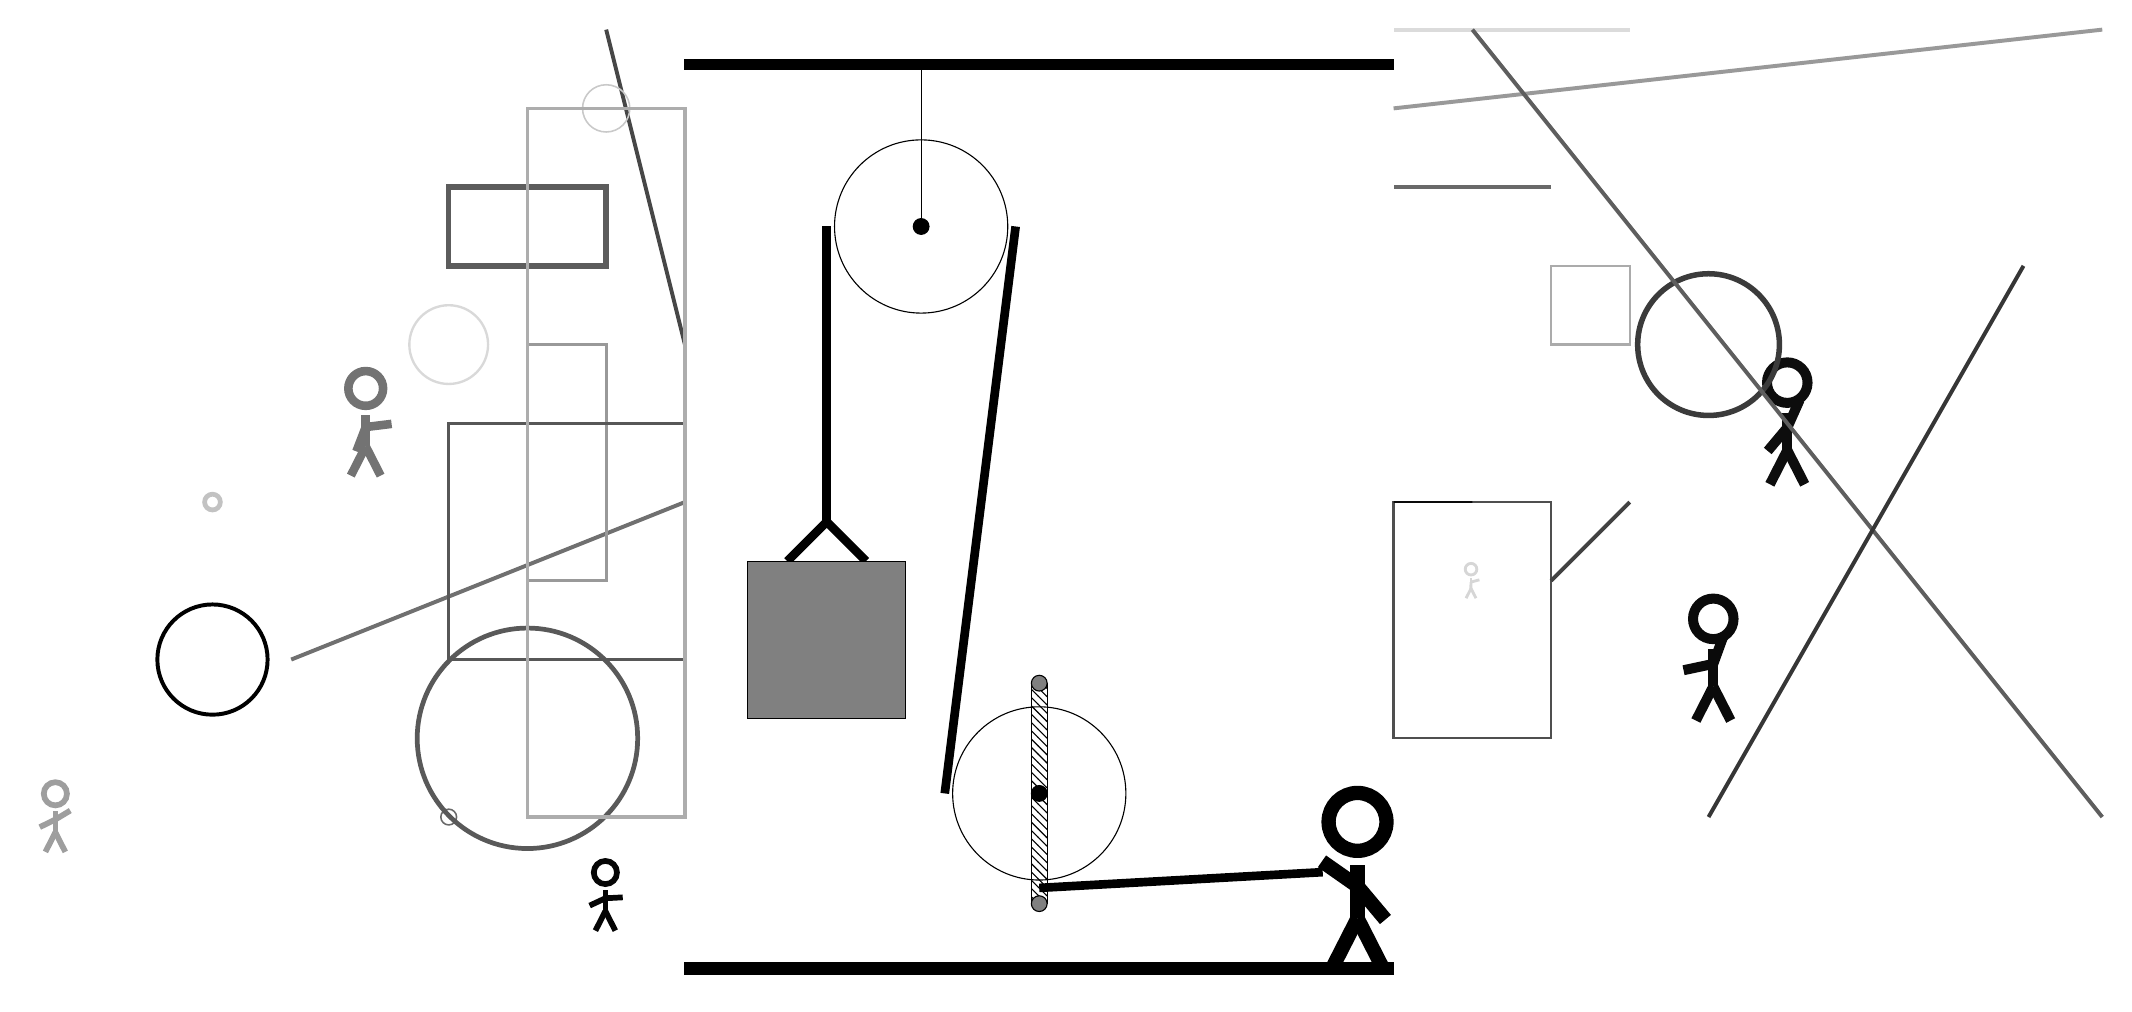
\begin{tikzpicture}
			%%%%% START %%%%%
			
			\draw[fill=black] (-2, 11.5) rectangle (7, 11.625);
			
			\draw (1, 9.5) circle (1.1);
			\draw[fill=black] (1, 9.5) circle (0.1);
			\draw (1, 11.5) -- (1, 9.5);
			
			\draw[fill=white](2.5, 2.3) circle (1.1);
			\draw[fill=black] (2.5, 2.3) circle (0.1);
			\draw[pattern=north west lines, pattern color=black] (2.4, 3.7) rectangle (2.6, 0.9);
			\draw[fill=black!50] (2.5, 3.7) circle (0.1);
			\draw[fill=black!50] (2.5, 0.9) circle (0.1);
			
			\draw[line width=1.1mm] (-0.7, 5.25) -- (-0.2, 5.75) -- (0.3, 5.25);
			\draw[fill=black!50] (-1.2, 5.25) rectangle (0.8, 3.25);
			
			\draw[line width=1.1mm] (-0.2, 9.5) -- (-0.2, 5.75);
			\centerarc[line width=1.1mm](1, 9.5)(0:180:1.2000000000000002);
			\draw[line width=1.1mm](2.2, 9.5) -- (1.3, 2.3);
			\centerarc[line width=1.1mm](2.5, 2.3)(180:270:1.2000000000000002);
			\draw[line width=1.1mm](2.5, 1.1) -- (6.1, 1.3);
			
			\node at (6.5, 1.2) {\Strichmaxerl[10][-35][-50]};
			
			\node[line width=0.5mm, color=black!96] at (11, 4) {\Strichmaxerl[7][12][70]};
			
			\draw[line width=0.3mm, color=black!69] (9, 3) rectangle (7, 6);
			\draw [line width=0.6mm, color=black!24](-8, 6) circle (0.1);
			\draw[line width=0.5mm, color=black!56](-2, 6) -- (-7, 4);
			
			\draw[line width=0.5mm, color=black!74](9, 5) -- (10, 6);
			\draw [line width=0.2mm, color=black!59](-5, 2) circle (0.1);
			\draw[line width=0.4mm, color=black!40] (-4, 8) rectangle (-3, 5);
			\draw[line width=0.5mm, color=black!40](7, 11) -- (16, 12);
			\draw[line width=0.5mm, color=black!59](9, 10) -- (7, 10);
			
			\draw [line width=0.5mm, color=black!100](-8, 4) circle (0.7);
			
			\draw[line width=0.5mm, color=black!72](-2, 8) -- (-3, 12);
			\draw[line width=0.5mm, color=black!77] (-2, 6) rectangle (-2, 7);
			\node[line width=0.7mm, color=black!98] at (-3, 1) {\Strichmaxerl[4][25][3]};
			
			\draw [line width=0.6mm, color=black!65](-4, 3) circle (1.4);
			\draw[line width=0.5mm, color=black!14](10, 12) -- (7, 12);
			\draw[line width=0.4mm, color=black!66] (-2, 4) rectangle (-5, 7);
			\node[line width=0.6mm, color=black!95] at (12, 7) {\Strichmaxerl[7][50][66]};
			\draw [line width=0.7mm, color=black!77](11, 8) circle (0.9);
			\node[line width=0.6mm, color=black!16] at (8, 5) {\Strichmaxerl[2][88][15]};
			
			\node[line width=0.5mm, color=black!55] at (-6, 7) {\Strichmaxerl[6][69][7]};
			\draw[line width=0.3mm, color=black!96] (7, 6) rectangle (8, 6);
			
			\draw[line width=0.7mm, color=black!64] (-3, 10) rectangle (-5, 9);
			\draw[line width=0.5mm, color=black!63](8, 12) -- (16, 2);
			\node[line width=0.2mm, color=black!38] at (-10, 2) {\Strichmaxerl[4][26][31]};
			\draw [line width=0.2mm, color=black!21](-3, 11) circle (0.3);
			
			\draw[line width=0.3mm, color=black!33] (9, 9) rectangle (10, 8);
			
			\draw [line width=0.3mm, color=black!15](-5, 8) circle (0.5);
			\draw[line width=0.4mm, color=black!32] (-4, 2) rectangle (-2, 11);
			
			\draw[line width=0.5mm, color=black!79](11, 2) -- (15, 9);
			
			\draw[fill=black] (-2, 0) rectangle (7, 0.15);
			
			%%%%% END %%%%%
		\end{tikzpicture}
	\end{figure}	
\end{document}